\documentclass[11pt,a4paper, swedish
]{article}
\pdfoutput=1

\usepackage{custom_as}
\graphicspath{ {figurer/} }

%%Drar in tabell och figurtexter
\usepackage[margin=10 pt, size=small]{caption}
%%För att lägga in 'att göra'-noteringar i texten
\usepackage{todonotes} %\todo{...}

%%För att själv bestämma marginalerna. 
\usepackage[
%            top    = 3cm,
%            bottom = 3cm,
%            left   = 3cm, right  = 3cm
]{geometry}

%%För att ändra hur rubrikerna ska formateras
%\renewcommand{\thesection}{...}


\newcommand{\PP}[1]{\ensuremath\mathcal{P}\left(#1\right)}

\newcommand{\VAR}[1]{\ensuremath\text{var}\!\left[#1\right]}


%%%%%%%%%%%%%%%%%%%%%%%%%%%%%%%%%%%%%%%%%%%%%%%%%%%%%%%%%%%%%%%%%%%%%%
\newcounter{exempel_counter}%[section]
\newenvironment{exempel}
{
  \refstepcounter{exempel_counter}
  \begin{quote}
  \noindent\textbf{Exempel~\arabic{exempel_counter}:}
}{
  \end{quote}
}
%%%%%%%%%%%%%%%%%%%%%%%%%%%%%%%%%%%%%%%%%%%%%%%%%%%%%%%%%%%%%%%%%%%%%%




\begin{document}
%\newgeometry{top=1cm, bottom=2cm}
%%%%%%%%%%%%%%%%% vvv Inbyggd titelsida vvv %%%%%%%%%%%%%%%%%
\title{\huge Behandling av experimentella resultat\\[2mm] 
\Large En introduktion för fysikstudenter om hur man ska\\ hantera
mätresultat och feluppskattningar}
\author{
Andréas Sundström\footnote{
\href{mailto:sundstrom.andreas@gmail.com}{\nolinkurl{sundstrom.andreas@gmail.com}}
\: Jag tar gärna emot synpunkter och förslag.}
}
\date{\today, \quad\texttt{v\,1.1}}
\maketitle

%%%%%%%%%%%%%%%%% ^^^ Inbyggd titelsida ^^^ %%%%%%%%%%%%%%%%%



\noindent{\bf\large Förord}\\[1mm]
\small
Det här kompendiet är skrivet som en introduktion i experimentella
mätningar, med fokus på feluppskattningar, för det svenska
IPhO-laget. Jag har försökt fatta mig kort, men jag har en tendens att
kunna dra iväg när jag skriver. Jag har försökt lägga innehållet på en
nivå för att kunna förstås av en gymnasieelev, men det är inte alltid
det går så bra\ldots{} Ni är de första som läser det här
kompendiet. Tycker du att det det här var för svårförståeligt så har
\textbf{jag} skrivit för komplicerat, och du är inte ensam om att
tycka att kompediet var svårt. \emph{Så säg till om det var krångligt!} 

Huvuddelen av kompendiel börjar med ett par punkter om vett och
etikett för experimentella problem. 
Sedan kommer huvudinnehållet, med felanalys och regression, i
avsnitt~\ref{sec:matfel}--\ref{sec:regression}. 
Men jag tyckte att det även kunde vara intressant med en liten
teoretisk bakgrund till varför man gör felanalysen som man gör
den. Bakgrunden finns i avsnitt~\ref{sec:statistik}, men man behöver
inte läsa det för att hänga med i resten av kompendiet.
Avslutningsvis räknas ett par exempel, med lite feluppskattning och
regresion/linjärisering, i avsnitt~\ref{sec:exempel}

Sedan har jag även lagt till en bilaga om
Taylorutvecklingar. Den hör inte så mycket ihop med resten av det här
kompendiet, men det är matnyttigt att kunna göra uppskattningar både
för teoretiska och experimentella beräkningar. 

\begin{flushright}
Andréas Sunsdtröm\\ 
Göteborg, 2016-06-16
\end{flushright}
\normalsize


\thispagestyle{empty}
\clearpage
\thispagestyle{empty}
\tableofcontents
\clearpage
\setcounter{page}{1}



\setcounter{section}{-1}
\section{Sannolihetslära och statistik (överkurs)}\label{sec:statistik}
När man gör mätningar vill man oftast ta reda på någon storhets värde
-- exempelvis periodtiden på en pendel. Med endast en mätning kan man
dock inte säga något om hur bra mätningen var. Men med flera mätningar
kan vi börja göra statistik över dem. Då kan man börja uppskatta hur
säker man kan vara på ens resutat.

Jag vill även betona vikten av statistik i framtida vetenskapliga och
tekniska karriärer. \emph{Statistik är ett mycket kraftfullt verktyg.}
Statistiken, när man börjar behärska den, är mycket mer än bara
''medelvärden och standardavvikelser''; den spelar en väsentlig roll i
mer eller mindre all experimentell vetenskap -- särskilt vid
feluppskattningar. 

\subsection{Stokastiska variabler}
Precis som vanliga variabler används stokastiska variabler för att
beteckna något okänt. Men i fallet med stokastiska variabler saknar de
ett värde. De är mer tänkta som ett koncept för att betecka en
slumpartad händelse eller process. Man kan göra en observation/mätning
av en stokastisk variabel och få ett värde, men det är bara ett ensilt 
mätvärde som man får och inte den stokastiska variabelns värde. 

\begin{exempel}
Ett tärningskast är ett exempel som kan beskrivas med en (diskret)
stokastisk variabel. Låt den stokastiska variabeln $X$ beskriva
tärningskastet. Den kan då mätas till ett visst utfall 
$x$. I fallet med tärningen $X$ finns ett utfallsrum som består av
talen 1 till 6: $\{1, 2, 3, 4, 5, 6\}$. Varje element i utfallsrummet
har också en viss sannolikhet, $\nicefrac{1}{6}$ i det här fallet.
 
Själva variablen $X$ (tärningen) kan alltså inte i sig ha ett värde.
Men när man gör en observation (kastar tärningen) kan man få ett
mätresultat $x$, som (när tärningen är kastad) har ett fast värde för
just det kastet. 
\end{exempel}

Fördelen med att ha stokastiska variabler är att man, likt vanliga
variabler, kan börja räkna med dem mer generellt än om man bara har
vissa specialfall. I det här avsnittet kommer de att användas för att
uttrycka statistiska och stokastiska samband, men det läggs inte så
stor vikt vid dem. 

\subsection{Sannolikhetsfördelningar och täthetsfunktioner}
Den statistik och sannolikhetslära man får lära sig i gymnasiet brukar
för det mesta vara diskret (och ändlig). Alltså att det finns ett
ändligt antal möjliga utfall och varje utfall är distinkt. Exempel på
detta är tärningskast, lottdragning och kortlekar. 

Verkligheten är dock oftast mer komplicerad än så. När man gör
mätningar handlar det oftas om mätnigar av en reellvärd storhet som
t.ex. en längd\footnotemark{}. Detta betyder att längden kommer att
anta ett reellt antal milimetrar och inte vara begränsad till ett
ändligt antal möjliga värden. För att analysera detta behövs statistik
för kontinuerliga fördelningar.  
\footnotetext{''Aha!'' tänker ni: atomer och kvantfysik gör att det
  bara finns diskreta längder. ''Nähä!'' säger jag: som fysiker måste
  man kunna hantera approximationer och veta begränsningarna i sina
  mätningar. Med en linjal eller skujtmått finns det ingen chans i
  världen att man skulle kunna stöta på problem orsakade av
  kvantfysik. Man kan alltså betrakta det som om de möjliga värden
  som längden kan anta ligger kontinuerligt.}

Sannolikhetsfördelningar karakteriseras av sin täthetsfunktion, som
brukar betecknas~$f$. Täthetsfunktionen talar om hur sannolikt det är
att få ett värde i ett visst intervall. Notera dock att den
\emph{inte} ger sannolikheten att få ett specifikt värde. 
Eftersom det finns (ouppräknerligt) oändligt många möjliga utfall så
är sannolikheten att få ett visst exakt värde
\begin{equation}
\PP{X=x}\; \text{''=''}\; \frac{1}{\infty}\; \text{''=''}\;0.
\end{equation}
För att istället beräkna sannolikheten att få sitt utfall $X$ i ett
visst intervall $[a, b]$ måste man integrera:
\begin{equation}\label{eq:dist_P}
\PP{a<X<b} = \int_a^b f(x) \id{x}.
\end{equation}
Sannolikheten att få $a<X<b$ bestäms alltså av arean under $f(x)$.

\begin{exempel}
Sannolikheten för att en radioaktiv kärna ska sönderfalla kan
beskrivas med den så kallade exponentialfördelningen:
\begin{equation*}
f(t)=
\begin{cases}
\lambda\ee^{-\lambda t},& t>0\\
0 ,& t\le0,
\end{cases}
\end{equation*}
där $\lambda$ är en konstant som kallas isotopens
sönderfallskonstant. 
Vad är sannolikheten att kärnan har sönderfallit vid tiden
$\tau=\nicefrac{\ln(2)}{\lambda}$? 

Sannolikheten att en kärna sönderfaller mellan tiden $0$ och $\tau$
ges enligt \eqref{eq:dist_P} helt enkelt av integralen
\begin{equation*}
\PP{0<T_\text{sönderfall}<\tau} 
= \int_0^\tau\lambda\ee^{-\lambda t}\id{t} 
= \lambda\,\frac{\ee^{0}-\ee^{-\lambda \tau}}{\lambda}
= 1-\ee^{-\lambda \tau}
=1-\frac{1}{2} = \frac{1}{2}.
\end{equation*}
Tolkningen av detta är att om man har väldigt många kärnor, så kommer
hälften av dem att ha sönderfallit vid tiden
$\nicefrac{\ln(2)}{\lambda}$. Detta är alltså vad man kallar isotopens
\emph{halveringstid}.
\end{exempel}



\subsubsection{Normalfördelningen}
En av de vanligaste fördelningarna är normalfördelningen. Den
har täthesfunktionen
\begin{equation}
f(x) = \frac{1}{\sqrt{2\pi\sigma^2}} \, \ee^{-\frac{(x-\mu)^2}{2\sigma^2}},
\end{equation}
där $\mu$ kallas fördelningens \emph{väntevärde} och $\sigma$ är dess
\emph{standardavvikelse}. I \figref{fig:normal_dist} visas
täthetsfunktionen för några olika val av $\mu$ och $\sigma$. Där ser
vi att $\mu$ svarar mot var någonstans fördelnigen är centrerad, och
att $\sigma$ svarar mot hur bred fördelningen blir. 

% Som kan ses i \figref{fig:normal_dist} går sannolikhetsfördelningen
% ner och blir väldigt liten för värden långt ifrån $\mu$. Till exempel
% ligger ca 98\,\% av all sannolikhet/area under kurvan inom $\mu\pm
% 2\sigma$, men sen går det snabbt -- fortsätter man uppåt så ligger
% 99,99997\,\% inom $\mu\pm 5\sigma$.

\begin{figure}
\centering
% GNUPLOT: LaTeX picture with Postscript
\begingroup
  \makeatletter
  \providecommand\color[2][]{%
    \GenericError{(gnuplot) \space\space\space\@spaces}{%
      Package color not loaded in conjunction with
      terminal option `colourtext'%
    }{See the gnuplot documentation for explanation.%
    }{Either use 'blacktext' in gnuplot or load the package
      color.sty in LaTeX.}%
    \renewcommand\color[2][]{}%
  }%
  \providecommand\includegraphics[2][]{%
    \GenericError{(gnuplot) \space\space\space\@spaces}{%
      Package graphicx or graphics not loaded%
    }{See the gnuplot documentation for explanation.%
    }{The gnuplot epslatex terminal needs graphicx.sty or graphics.sty.}%
    \renewcommand\includegraphics[2][]{}%
  }%
  \providecommand\rotatebox[2]{#2}%
  \@ifundefined{ifGPcolor}{%
    \newif\ifGPcolor
    \GPcolortrue
  }{}%
  \@ifundefined{ifGPblacktext}{%
    \newif\ifGPblacktext
    \GPblacktexttrue
  }{}%
  % define a \g@addto@macro without @ in the name:
  \let\gplgaddtomacro\g@addto@macro
  % define empty templates for all commands taking text:
  \gdef\gplbacktext{}%
  \gdef\gplfronttext{}%
  \makeatother
  \ifGPblacktext
    % no textcolor at all
    \def\colorrgb#1{}%
    \def\colorgray#1{}%
  \else
    % gray or color?
    \ifGPcolor
      \def\colorrgb#1{\color[rgb]{#1}}%
      \def\colorgray#1{\color[gray]{#1}}%
      \expandafter\def\csname LTw\endcsname{\color{white}}%
      \expandafter\def\csname LTb\endcsname{\color{black}}%
      \expandafter\def\csname LTa\endcsname{\color{black}}%
      \expandafter\def\csname LT0\endcsname{\color[rgb]{1,0,0}}%
      \expandafter\def\csname LT1\endcsname{\color[rgb]{0,1,0}}%
      \expandafter\def\csname LT2\endcsname{\color[rgb]{0,0,1}}%
      \expandafter\def\csname LT3\endcsname{\color[rgb]{1,0,1}}%
      \expandafter\def\csname LT4\endcsname{\color[rgb]{0,1,1}}%
      \expandafter\def\csname LT5\endcsname{\color[rgb]{1,1,0}}%
      \expandafter\def\csname LT6\endcsname{\color[rgb]{0,0,0}}%
      \expandafter\def\csname LT7\endcsname{\color[rgb]{1,0.3,0}}%
      \expandafter\def\csname LT8\endcsname{\color[rgb]{0.5,0.5,0.5}}%
    \else
      % gray
      \def\colorrgb#1{\color{black}}%
      \def\colorgray#1{\color[gray]{#1}}%
      \expandafter\def\csname LTw\endcsname{\color{white}}%
      \expandafter\def\csname LTb\endcsname{\color{black}}%
      \expandafter\def\csname LTa\endcsname{\color{black}}%
      \expandafter\def\csname LT0\endcsname{\color{black}}%
      \expandafter\def\csname LT1\endcsname{\color{black}}%
      \expandafter\def\csname LT2\endcsname{\color{black}}%
      \expandafter\def\csname LT3\endcsname{\color{black}}%
      \expandafter\def\csname LT4\endcsname{\color{black}}%
      \expandafter\def\csname LT5\endcsname{\color{black}}%
      \expandafter\def\csname LT6\endcsname{\color{black}}%
      \expandafter\def\csname LT7\endcsname{\color{black}}%
      \expandafter\def\csname LT8\endcsname{\color{black}}%
    \fi
  \fi
  \setlength{\unitlength}{0.0500bp}%
  \begin{picture}(6802.00,3968.00)%
    \gplgaddtomacro\gplbacktext{%
      \csname LTb\endcsname%
      \put(946,704){\makebox(0,0)[r]{\strut{} 0}}%
      \csname LTb\endcsname%
      \put(946,1454){\makebox(0,0)[r]{\strut{} 0.1}}%
      \csname LTb\endcsname%
      \put(946,2204){\makebox(0,0)[r]{\strut{} 0.2}}%
      \csname LTb\endcsname%
      \put(946,2953){\makebox(0,0)[r]{\strut{} 0.3}}%
      \csname LTb\endcsname%
      \put(946,3703){\makebox(0,0)[r]{\strut{} 0.4}}%
      \csname LTb\endcsname%
      \put(1078,484){\makebox(0,0){\strut{}-6}}%
      \csname LTb\endcsname%
      \put(1966,484){\makebox(0,0){\strut{}-4}}%
      \csname LTb\endcsname%
      \put(2854,484){\makebox(0,0){\strut{}-2}}%
      \csname LTb\endcsname%
      \put(3742,484){\makebox(0,0){\strut{} 0}}%
      \csname LTb\endcsname%
      \put(4629,484){\makebox(0,0){\strut{} 2}}%
      \csname LTb\endcsname%
      \put(5517,484){\makebox(0,0){\strut{} 4}}%
      \csname LTb\endcsname%
      \put(6405,484){\makebox(0,0){\strut{} 6}}%
      \put(176,2203){\rotatebox{-270}{\makebox(0,0){\strut{}$f(x)$}}}%
      \put(3741,154){\makebox(0,0){\strut{}$x$}}%
    }%
    \gplgaddtomacro\gplfronttext{%
      \csname LTb\endcsname%
      \put(2530,3475){\makebox(0,0)[r]{\strut{}$\mu=0$, $\sigma=1$}}%
      \csname LTb\endcsname%
      \put(2530,3255){\makebox(0,0)[r]{\strut{}$\mu=0$, $\sigma=2$}}%
      \csname LTb\endcsname%
      \put(2530,3035){\makebox(0,0)[r]{\strut{}$\mu=2$, $\sigma=1$}}%
    }%
    \gplbacktext
    \put(0,0){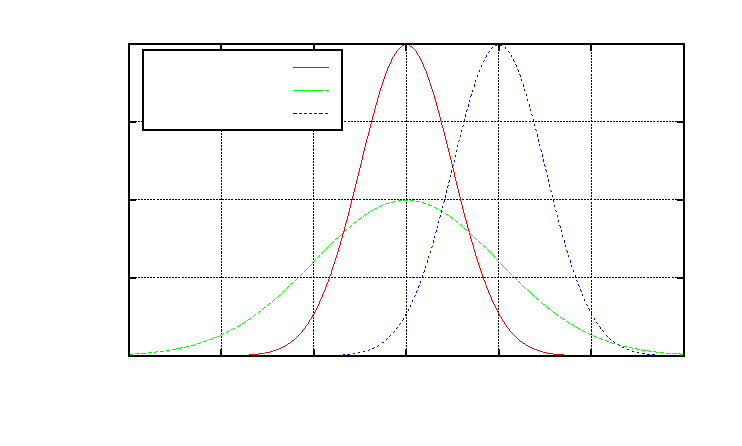
\includegraphics{normal_dist}}%
    \gplfronttext
  \end{picture}%
\endgroup

\caption{Täthetsfunktioner till normalfördelningar med olika värden på
väntevärdet $\mu$ och standardavvikelsen $\sigma$. Varje kurva har den
klassiska Gau\ss{}iska klockformen.}\label{fig:normal_dist}
\end{figure}

Kvadraten i exponentialen ger täthetsfunktionen den
klassiska klockformen hos en Gau\ss{}isk kurva, och faktorn framför
säkerställer att den totala integralen
\begin{equation}
\int_{-\infty}^{\infty} f(x)\id{x} = 1.
\end{equation}
Detta är något som \emph{gäller för alla täthetsfunktioner}. 

Normalfördelningen kallas just ''normal'' för att det finns en sats
som säger att i princip alla slumpfenomen blir normalfördelade om
samma process upprepas väldigt många gånger. Ett exempel på detta är
om man sannolikheten att få ett visst antal ''klave'' efter flera
slantsinglingar. Den här egenskapen gör att de allra flesta 
mätfelen antas vara normalfördelade.

% Vidare är normalfördelningen en väldigt trevlig fördelning att arbeta
% med. Regeln för normalfördelningar är att om $X$ och $Y$ båda är
% normalfördelade och oberoende med väntevärde $\mu_X$ och
% standardavvikelse $\sigma_X$ respektive $\mu_Y$ och $\sigma_Y$, så är 
% \begin{equation}
% Z=\alpha X + \beta Y
% \end{equation}
% också normalfördelad med väntevärde $(\alpha\mu_X+\beta\mu_Y)$ och
% standardavvikelse $\sqrt{\alpha^2\sigma_X^2 + \beta^2\sigma_Y^2}$. 
% Med andra ord funkar väntevärdena som man kan tro och
% standardavvikelserna fungerar lite som Pythagoras sats. 


\subsection{Väntevärden, varianser och standradavvikelser}
De vanligaste fördelningarna har, som normalfördelningen, väntevärde
och varians. Dessa beräknas med hjälp av täthetsfunktionen. I
felanalys används främst den så kallade standardavvikelsen, som 
är roten ur variansen.

Väntevärdet av den stokastiska variabeln $X$, med täthetsfunktion $f$,
definieras som 
\begin{equation}\label{eq:ev}
\ev{X} = \mu = \int_{-\infty}^\infty x f(x)\id{x}.
\end{equation}
Det är inte helt kart vad tolkningen ska vara direkt från
definitionen, men man kan jämföra väntevärdesintegralen med en slags
tyngdpunktsberäkning. Man lägger ihop varje punkts
''sannolikhetsmassa'', $f(x)\dd{x}$, gånger punktes avstånd, $x$, från
origo; till slut får man den sammanlagda tyngdpunkten. Man kan
faktiskt, om man vill, hitta en fördelnings väntevärde genom att kippa
ut en (styv) pappersbit formad efter ytan under kurvan och balanseta
den utklippta formen. 

Sedan kan variansen definieras med hjälp av väntevärden:
\begin{equation}\label{eq:var}
\VAR{X} = \sigma^2 =\ev{(X-\mu)^2}. %\ev{X^2} - \mu^2.
\end{equation}
%Det sista ledet ovan är ett sätt som man kan skriva om variansen, men
%det används mest i teoretiska analyser och är inte så viktigt i
%nuläget. 
Tolkningen av variansen är att det är ett väntevärde på hur
mycket avvikelse man får från $\mu$, men för att inte positiva
och negativa avvikelser ska ta utvarandra, kvadreras de innan man tar
väntevärdet. Detta ger dock ett mått som är
''kvadratiskt''\footnotemark{}, så för att få något som kan jämföras
med själva värdena man får från $X$ använder man
\emph{standardavvikelsen som är roten ur variansen}. 
\footnotetext{Om till exempel $X$ är en sorts längd, med enhet meter,
  bli $\VAR{X}$ en storhet som är en längd i kvadrat, med enhet
  kvadratmeter. }

\subsubsection{Några nyttiga satser}\label{sec:satser}
Det viktigaste man behöver veta om väntevärden är att de är
linjära. Alltså att
\begin{equation}\label{eq:ev_lin}
\Big\langle \alpha X + \beta Y + \gamma \Big\rangle 
= \alpha\ev{X} + \beta\ev{Y} + \gamma,
\end{equation}
för godtyckliga stokastiska variabler $X$ och $Y$ samt några
konstanter $\alpha$, $\beta$ och $\gamma$. Den här regen kan utvidgas
till ett godtyckligt antal variabler. 

För variansen gäller en liknande regel 
\begin{equation}\label{eq:var_lin}
\text{var}\!\Big[ \alpha X + \beta Y + \gamma \Big] 
= \alpha^2\VAR{X} + \beta^2\VAR{Y}, 
\end{equation}
men här måste $X$ och $Y$ vara statistiskt
oberoende\footnotemark{}. Även här kan man utvidga regeln till ett
godtyckligt antal oberoende variabler.
\footnotetext{Statistiskt oberoende är en ganska knepig term att
  deffiniera. Men enkelt sett så betyder det ungefär vad magkänslan
  säger: att resultatet av en mätning på den ena ska inte påverka
  resultatet på den andra. }

Speciellt gäller att om man har $N$ stycken oberoende stokastiska variabler
$X_i$ med lika fördelning och man vill ta ett medelvärde 
\begin{equation} 
\bar{X} = \frac{X_1+X_2+\cdots+X_N}{N} = \frac{1}{N}\sum_{i=1}^N X_i
\end{equation}
så kan man beräkna dess väntevärde och varians med hjälp av reglerna
ovan. 
Väntevärdet ges då från \eqref{eq:ev_lin} som
\begin{equation}\label{eq:ev_mean}
\ev{\bar{X}} = \ev{\frac{1}{N} \sum_{i=1}^N X_i} 
= \frac{1}{N} \sum_{i=1}^N \overbrace{\ev{X_i}}^{=\mu} 
= \mu,
\end{equation}
där $\mu$ är väntevärdet av varje enskild variabel från den givna
fördelningen. 
Variansen får man med \eqref{eq:var_lin} sedan som
\begin{equation}\label{eq:var_mean}
\VAR{\bar{X}} = \VAR{\frac{1}{N} \sum_{i=1}^N X_i}
= \VAR{\sum_{i=1}^N \frac{1}{N} X_i}
= \sum_{i=1}^N \frac{1}{N^2}\overbrace{\VAR{X_i}}^{=\sigma^2}
= \frac{\sigma^2}{N}.
\end{equation}

Dessa resultat kommer att användas i feluppsattningar genom att
betrakta varje $X_i$ som en mätning av en viss storhet.

\subsubsection{Skattning från mätdata}
Har man ett stokastiskt system och vill försöka mäta dess väntevärde
och standardavvikelse, så måste man ha många mätningar på det. Det är
nu som statistiken kommer in i bilden.

Från \eqref{eq:ev_mean} visade det sig att väntevärdet av ett
medelvärde är samma som väntevärdet av det man mäter på. Vidare visade
det sig att variansen av medelvärdet minskade som
$\nicefrac{1}{N}$. Tillsammans ger detta att \emph{ju fler mätningar
  man gör desto större är sannolikheten att medelvärdet ligger nära
  väntevärdet}. 
Detta betyder att man kan skatta väntevärdet med
\begin{equation}\label{eq:ev_approx}
\ev{X} = \mu \approx \bar{x} = \frac{1}{N}\sum_{i=1}^N x_i.
\end{equation}
Här användes små bokstäver $x_i$ för att beteckna att de redan är
uppmätta värden.

Om nu väntevärden gick att skatta som medelvärden bör man väl kunna
göra det samma för varianser. Definitionen av varians i \eqref{eq:var}
består ju av två väntevärden (två stycken eftersom $\mu=\ev{X}$), så
det borde gå att skatta variansen med medelvärdet av
$(x_i-\bar{x})^2$. Svaret är att det  nästan går. Eftersom man bara
får ett ungefärligt värde på $\mu$ från \eqref{eq:ev_approx} måste
medelvärdet justeras något. Det visar sig att man ska använda
\begin{equation}\label{eq:var_approx}
\VAR{X} = \sigma^2 \approx s^2 = \frac{1}{N-1}\sum_{i=1}^N (x_i-\bar{x})^2
\end{equation}
för att skatta variansen. Standardavvikelsen fås enkelt genom att dra
roten ur skattningen av variansen:
\begin{equation}\label{eq:std_approx}
\sigma \approx s = \sqrt{\frac{1}{N-1}\sum_{i=1}^N (x_i-\bar{x})^2}.
\end{equation}
Detta kallas \emph{standradfelet} och är det namn som man har gett
till skattningen av standardavvikelsen.
Notera att $s$ är standradfelet i uppsättnigen av alla
mätpunkter. För att få \emph{standardfelet i medelvärdet}
använder man \eqref{eq:var_mean} och får $\nicefrac{s}{\sqrt{N}}$.






\newpage
\section{Innan man börjar felanalysen}
Det finns ett par saker som är bra att tänka på innan, under och efter
man börjar göra sina mätningar.
\begin{itemize}
\item \emph{Vad behöver jag mäta?} Det är alltid bra att tänka igenom
  vilka samband som gäller och vilka parametar som behöver mätas. Allt
  detta för att slippa göra om en mätning i onödan eller behöva göra
  en ny mätning.
\item \emph{Vad förväntar jag mig att få som resultat?} Det är inte
  alltid det går att uppskatta vad man borde få för resultat, men i de
  fall där man faktiskt kan göra det är det bra om man kan lägga några
  minuter på att uppskatta vad man borde få för resultat. 
\item \emph{Var behöver jag mäta?} När man håller på och tar upp en
  mätserie är det dumt att hålla på och ta upp punkter som ligger
  onödigt tätt. Det är oftast bättre att börja med att gå igenom
  mätintervallet med ganska stora steg och notera var de
  intressanta ställena ligger; sen kan du gå tillbaks dit och ta några
  fler mätpunkter där. (I IPhO brukar de vilja att man tar minst
  10~mätpunkter i en serie.)
\item \emph{Blev någon mätning dålig?} Det är okej att slänga bort
  enstaka mätvärden som är väldigt utstickande. Titta över era
  mätningar och se om någon mätpunkt verkar ligga långt ifrån det
  förväntade innan ni börjar med den övriga dataanalysen. (I mätningar
  i en mätserie kan man behöva plotta ut sina mätpunkter innan man kan
  hitta någon avvikelse.)
\item \emph{Verkar slutresultatet rimligt?} Utöver enskilda mätvärden
  bör man också titta på det slutgiltiga resultatet och se om det
  verkar stämma. (Om svaret verkar helt tokigt, säg det! Ibland kanske
  det går att få till förmildrande omständigheter om man påpekar att
  det verkar fel.)
\item \emph{Hur ska resultatet presenteras?} Kolla över
  uppgiftspapprena för att se hur svaret till varje deluppgit ska
  presenteras.
  \begin{itemize}
  \item OBS: Glöm inte \textbf{enheter!} (Det gäller allt:
  tabellhuvuden, axler till grafer, uträkningar på pappret och så
  klart i svaret.)
  \item Tänk på hur många värdesiffror det är rimligt att ta
    med. (Det kan ge poängavdrag i IPhO att ta med för många, eller
    för få, värdesiffror.)
  \end{itemize}
\end{itemize}

\section{Olika typer av mätfel}\label{sec:matfel}
När man vill uppskatta hur stora experimentella fel/osäkerheter man
har finns det två typer av fel och två typer av feluppskattningar. De
två typerna av fel som finns är systematiska och statistiska. Sedan är
de två typerna av feluppskattningar som man behöver kunna. Dels direkt
feluppskattning (av statistiska fel), dels propagering av osäkerhet. 

I det här avsnittet presenteras de två typerna av fel och direkt
feluppskattning. Efter detta kommer nästa avsnitt att handla om
felpropagering. 


\subsection{Systematiska fel -- noggrannhet och precision}
\begin{figure}
\centering
\resizebox{0.5\textwidth}{!}{
\input{figurer/precision_noggrannhet.pdf_t}
}
\caption{Illustration av skillnaden mellan noggrannhet och
  precision. Måltavlorna representerar en mätning, där mitten på
  måltavlan svarar mot det ''sanna'' värdet. Fallen med låg
  noggrannhet svarar mot systematiska fel som inte går att avhjälpa
  med medelvärden av fler mätningar.}
\label{fig:prec_nog}
\end{figure}

Ett systematiskt fel är något som gör att ens mätresultat hela tiden
är lite fel åt något håll\footnotemark{}. Dessa karakteriseras av att
det inte hälper med flera mätningar för att få bättre mätresultat.
\footnotetext{Det behöver inte nödvändigtvis vara så att det är just
  fel åt samma håll hela tiden, men oftast är ett systematiskt fel
  något som ger en förskjutning av ens mätresultat.}

Man brukar skilja på två olika typer av godhet i mätningar. Det finns
dels noggrannhet, dels precision. Noggrannhet, eller rikighet som det
ibland kallas, svarar mot hur nära det ''sanna''\footnotemark{} värdet
mätningarna kommer i medel. Prescisionen svarar å andra sida mot hur
tätt mätresultaten hamnar, eller hur liten spridning man får i dem. De
två koncepten illustreras i \figref{fig:prec_nog}.  
\footnotetext{Jag sätter ''sanna'' inom citationstecken för att ur ett
experimentalistiskt perspektiv finns det inget sätt att veta det
verkligt sanna värdet -- man kan bara se var man träffade men inte
måltavlan. Detta gör att det inte går att säga att man har fått det
sanna värdet. }

Som kan ses i \figref{fig:prec_nog} svarar låg noggrannhet mot ett
systematiskt fel som gör att medelvärdet avviker från det ''sanna''
värdet. Vidare kan man med statistisk analys bara ta reda på
spridningen i resultaten -- alltså hur bra precision man
har. Tillsammans ger detta en ganska prekär situation att hantera i
felanalys: 
\emph{Man vill veta hur {\bf noggranna} ens mätningar är, men man kan bara
  ta reda på hur {\bf precisa} de är.} 

Sättet man löser detta på är att låtsas som att det regnar och strunta
i eventuella systematiska fel när man redovisar sin felanalys. Detta
förutsätter såklart att man verkligen har försökt eliminera alla
systematiska fel; de som är kvar är dock de som man inte kände till,
vilket betder att det i princip är omöjligt att kunna uppskatta
storleken på dem. I praktiken redovisar man oftast bara spridingen i
mätresultaten och säger att märosäkerheten är samma som spridningen --
man antar alltså att det inte längre finns några systematiska fel. 

\subsubsection{Mätupplösning}
En sorts systematiska\footnotemark{} osäkerheter som man ofta kommer
att stöta på härör från mätinstrumentents upplösning. Ett exempel på
detta är en linjal; oavsett hur många gånger man försöker mäta bredden
på ett hårstrå kommer man bara att få 0\,mm som resultat. 
\footnotetext{Jag har valt att klassa dem som systematiska av
  anledningen att det oftast inte hjälper att ta ett medelvärde av
  flera mätningar. }

Sättet att hantera detta på är att erkänna att man har ett
systematiskt fel som kommer från upplösningen, och ta med det i
beräkningarna. Detta gör man genom att själv uppskatta vad
avrundningsfelet kan vara i mätningen. Generellt gäller att
\begin{itemize}
\item analoga intrument har ett avrundningsfel som är halva
  avståndet mellan markörer. Alltså att en linjal som är mm-graderad
  får en mätosäkerhet på $\pm\unit[0,5]{mm}$ (även om man tycker att
  mätninger ser ut att vara närmare skalstecket än så).
\item digitala intrument är ganska opålitliga i hur noggranna de
  är. Detta betyder att osäkerheten \emph{inte} behöver vara i sista
  siffran, utan man måste kolla manualen för att veta hur bra de är. 
  \emph{I IPhO gäller dock att man får anta att osäkerhetsgränsen
    ligger på ''plus-mius ett'' i den sista siffran.} 
\item tidtagning med tidtagarur har en osäkerhet på \emph{minst}
  $\pm\unit[0,1]{s}$ (även om tidtagaruret går ner till hundradels
  sekunder). Detta är helt enkelt för att den mänskliga reaktionstiden
  inte är snabbare än så. Dock är tidtagning något som typiskt lämpar
  sig väl för upprepade mätningar.
\end{itemize}

Dessa tumregler kan användas i fall där man bedömmer att upprepade
mätningar inte kommer att kunna ge förändrade mätresultat. Några (men
inte alla) typfall där detta gäller är längdmätning (av något objekt)
med linjal eller skjutmått, och spännings- eller strömmätningmätning
med multimeter. I andra fall är det alltid rekommenderat att göra
upprepade mätningar (gärna upp till 10 stycken men minst 3). 


\subsection{Statistiska osäkerheter och hur man uppskattar dem}
För att ta reda på precisionen i mätresultaten behövs statistik. Om
ens noggrannhet är hög (övre halvan i \figref{fig:prec_nog}) behöver
man ändå veta hur god precision man har. Gör man bara en mätning har
man ingen möjlighet att veta hur nära det ''sanna'' resultatet man
kom. Det är där man måste börja använda lite statistik. 

Säg att det finns en storhet $x$ som ska mätas, men att varje mätning
har ett mätfel~$\delta{x}$. Det som mäts blir då
\begin{equation}
\widetilde{x}_i=x+\delta{x}_i.
\end{equation}
Utan någon mer informationom $\delta{x}$ går det inte att säga så mycket mer
från mätningen. Men som sagts tidigare antas mätfelet $\delta{x}$ vara
normalfördelat med $\mu=0$ fast med ett okänt $\sigma$. Det är oftas
$\sigma$ som man tar reda på för att sen få en osäkerhetsuppskattning av
ens mätning. 

För att få fram ett värde på $x$ tar man ett medelvärdet av flera
mätningar. Detta ger
\begin{equation}
\bar{x}=\frac{\widetilde{x}_1+\widetilde{x}_2 + \cdots + \widetilde{x}_N}{N} 
= \frac{Nx+\delta{x}_1+\delta{x}_2 + \cdots + \delta{x}_N}{N}
= x + \overline{\delta{x}}.
\end{equation}
Vi utnyttjar nu att medelvärdet
$\overline{\delta{x}}\approx\mu=0$, vilket ger att $\bar{x}\approx x$.
Här syns att antagandet $\mu=0$ betydet att det inte finns något
systematiskt fel.

För att sedan ta reda på precisionen i mätningarna behövs
standardavvikelsen av $\delta{x}$. Denna fås enkelt som standradfelet
från \eqref{eq:std_approx}. Men eftersom det beräknade värdet
$\bar{x}$ är ett medelvärde betyder det att osäkerheten är mindre i
$\bar{x}$ än i varje enskilt $\widetilde{x}_i$. Standardfelet från
\eqref{eq:std_approx} ger däremot en mått på hur spridda värden man
har fått. Som nämnts tidigare får man standardavvikelsen i
\emph{medelvärdet} genom att dela med
$\sqrt{N}$. Mätosäkerheten\footnotemark{} $\Delta{x}$ blir då

{\Large
\begin{equation} \label{eq:Delta_x}
\Delta{x} = \frac{s}{\sqrt{N}} 
= \frac{1}{\sqrt{N}} \sqrt{\frac{1}{N-1}\sum_{i=1}^N (x_i-\bar{x})^2}.
\end{equation}
}
\footnotetext{Notera skilnaden mellan $\delta{x}$ och $\Delta{x}$. Den
första är felet i varje enskild mätning, medan den andra är är den
totala osäkerheten i slutresultatet av en längre märserie.}

Detta är en av de vanligaste beräkningarna man kommer att behöva göra
i felanalys. De räknare som används på IPhO kan därför ställas in för
att göra precis den här beräkningen, men bara nästan: man får $s$, sen
måste man själv dela med $\sqrt{N}$. Samtidigt känns det lite som fusk
att man bara kan ''slänga in ett extra $\sqrt{N}$ och så blev
osäkerheten plötsligt mindre''.\footnotemark{} Men matten i
avsnitt~\ref{sec:satser} visar att man ska göra det.
\footnotetext{
  Det här var en av de svåraste sakerna att acceptera med felanalys
  när jag började med sånt. Men allt följer från \eqref{eq:var_mean}.
}


\section{Felpropagering}
Oftast kan man inte mäta den eftersökta storheten direk. Man brukar
istället mäta ett antal andra storheter och utnyttja något teoretiskt
samband för att få värdet på den eftersökta storheten. Då kan man
utnyttja feluppskattningarna ovan för att ta reda på felet i varje
uppmätt värde. Men hur får man reda på osäkerheten i slutresultatet?
Det är här som man måste använda felpropagering. 

\subsection{Insättningsmetoden -- en inte så bra metod}
Man skulle kunna göra en insättning av största eller minsta möjliga
värde på de uppmätta storheterna i sambandet för att få ett största
eller minsta värde på slutresultatet. På så sätt kan man beräkna
mellan vilka värden slutresultatet skulle kunna variera, vilket ger en
uppskattning av osäkerheten i det.

\begin{exempel}\label{ex:fel_insattning}
Tänk er att ni vill mäta arean av en rektangel och att ni har fått
dess sidlängder som $a=\unit[5\pm1]{cm}$ och $b=\unit[8\pm2]{cm}$. Då
blir arean $\bar{A}=\unit[40]{cm^2}$. Men maximalt skulle den kunna vara
$A_\text{max}=\unit[6]{cm}\times\unit[10]{cm}=\unit[60]{cm^2}$ och minimalt
$A_\text{min}=\unit[4]{cm}\times\unit[6]{cm}=\unit[24]{cm^2}$, vilket skulle ge
en osäkerhet på $\hat\Delta{A}=\unit[(60-24)]{cm^2}=\unit[36]{cm^2}$. 
Detta är en \emph{väldig stor} osäkerhet.
\end{exempel}

Som exemplet visar så blev osäkerheten väldigt stor. Detta beror på
att max- och minvärdena beräknas genom att låta alla mätfel dra åt
samma håll. Alltså att både $a$ och $b$ togs till sina respektive max-
och minvärden för att beräkna areans max- och minvärde. 
\emph{Men mätfel antas vara slumpmässiga så det är inte särskilt sannolikt
att båda mätningarna var felaktiga ''åt samma håll''. }

\subsection{Linjärisering -- ett bättre sätt att göra det på}
Ett annat problem med insättningsmetoden är att den är ganska tidskrävande
att göra för hand. Då är det lättare att anta att felen är små och
använda en linjärapproximation (se bilaga~\ref{sec:Taylor}) av
sambandet för att uppskatta hur mycket slutvärdet ändrar sig om man
ändrar de uppmätta parametrarna något.

Låt säga att en storhet $G$ ska bestämmas genom något godtyckligt
samband 
\begin{equation}\label{eq:some_function}
G=G\big(x, y, z \big),
\end{equation}
där de uppmätta storheterna har varsina osäkerheter
$x=\bar{x}+\Delta{x}$, $y=\bar{y}+\Delta{y}$ och
$z=\bar{z}+\Delta{z}$. Då blir $\bar{G}=g(\bar{x}, \bar{y}, \bar{z})$,
men hur uppskattar man osäkerheten?

Börja med att anta att det bara finns fel i $x$ -- alltså att
$\Delta{y}=\Delta{z}=0$. Då ger en linjärapproximation att
\footnote{Derivator med krulliga d:n ($\pd$) används för funktioner av
  flera variabler, och betder att man deriverar funktionen med
  avsenende på endast en variabel och betraktar de andra som
  konstanter.}
\footnote{Jag sätter beloppstecken på derivatorna för att
  osäkerheterna $\Delta{G}$ och $\Delta{x}$ av konvension alltid är
  positiva.} 
\begin{equation}\label{eq:error_one_variable}
\frac{\Delta{G}}{\Delta{x}} \approx \abs{ \pdv{G}{x} } 
\quad\Longleftrightarrow\quad
\Delta{G} \approx \abs{ \pdv{G}{x} } \Delta{x}.
\end{equation}
Härifrån ses att $\Delta{x}$ måste vara ganska litet för att
approximationen ska vara tillförlitlig, men det är oftas inga problem. 


\begin{figure}
\centering
\input{figurer/3D.pdf_t}
\caption{Ett sätt att se på hur fel i flera inparametrar kan samverka
  för att skapa ett totalt fel i slutresultatet. Alla felen drar åt
  varsitt håll, men i varsin dimension. Detta gör att man får ett
  resulterande fel vars storkel kan beräknas med ''Pythagoras sats''.}
\label{fig:3D}
\end{figure}

Det här ska nu utvidgas till resten av variablerna. Detta görs genom
att använda det andra av de två uttrycken ovan. Bidragen från varje
invariabel bestäms på ett analogt sätt med hur det gjordes för bara
$x$. 
Men för att inte hamna i samma situation som med insättningsmetoden,
(att alla felen drar åt samma håll) räcker det inte med att addera
ihop felen från varje variabel. 
Man tänker sig istället ungefär att felen drar åt varisitt håll fast i
flera dimensioner som i \figref{fig:3D}. Det totala felet i
slutresultatet fås då som en slags ''Pythagoras sats'': 
\footnote{Beloppstecknen i \eqref{eq:error_one_variable} har
  försvunnit hät. Det är för att kvadraten ändå alltid är positiv. }

\Large
\begin{equation}\label{eq:error_main}
\Delta{G} \approx \sqrt{
\left(\pdv{G}{x}\Delta{x}\right)^2
+\left(\pdv{G}{y}\Delta{y}\right)^2
+\left(\pdv{G}{z}\Delta{z}\right)^2
}.
\end{equation}
\normalsize
När man beräknar ett propagerat fel med den här formeln ska man komma
ihåg att alla derivatorna ska beräknas med $x=\bar{x}$, $y=\bar{y}$
och $ z=\bar{z}$.
Det här uttrycket kan självklart utvidgas till vilket antal
invariabler som helst. 


\begin{exempel}
Nu kan vi beräkna osäkerheten på rektangelarean från det förra
exemplet. Eftersom $A=a\cdot b$ blir
\[
\pdv{A}{a}=b \quad\text{och}\quad \pdv{A}{b}=a,
\]
vilket med \eqref{eq:error_main} ger
\[
\Delta{A} = \sqrt{
\Big(\bar{b}\,\Delta{a}\Big)^2 \!+
\Big(\bar{a}\,\Delta{b}\Big)^2
}
= \sqrt{
\Big(\unit[8]{cm}\times\unit[1]{cm}\Big)^2 \!+
\Big(\unit[5]{cm}\times\unit[2]{cm}\Big)^2
}
= \unit[13]{cm^2}.
\]
Den här osäkerheten är betydligt mindre jämfört med det från insättningsmetoden:
$\hat{\Delta}{A}=\unit[36]{cm^2}$ från exempel~\ref{ex:fel_insattning}. 

Tittar man på de relativa\footnotemark{} osäkerheterna så ligger de på
20--25\,\% för $a$ och $b$, medan man får
${\Delta{A}}/{\bar{A}}=32\,\%$ respektive
${\hat{\Delta}{A}}/{\bar{A}}=90\,\%$ som relativ osäkerhet i
arean. Här verkar ju alternativet med 32\,\% stämma betydligt bättre
överens med hur stora fel vi hade från början. 
\footnotetext{En relativt osäkerhet är bara osäkerheten uttryckt i
  procent istället för absoluta värden.}
\end{exempel}


\subsubsection{Potenssamband}
Det kanske känns som att metoden i \eqref{eq:error_main} inte är
mycket enklare att använda än insättningsmetoden, men den här metoden har en
stor styrka: med rena potenssamband blir den väldigt enkel. Och ärligt
talat så är ganska många fysikaliska samband någon form av
potenssamband. 

Antag nu att sambandet i \eqref{eq:some_function} är ett
potenssamband:
\begin{equation}
G=G\big(x, y, z \big) = c\:x^\alpha\, y^\beta \,z^\gamma,
\end{equation}
där $c$, $\alpha$, $\beta$ och $\gamma$ är konstanter.
Då kan derivatorna skrivas
\begin{equation}
\pdv{G}{x} = c\,\alpha x^{\alpha-1}\, y^\beta \,z^\gamma = \alpha\, \frac{G}{x}
\end{equation}
och på samma sätt för $y$ och $z$. Detta ger att
\eqref{eq:error_one_variable} kan skrivas om till 
(med $\Delta{y}=\Delta{z}=0$) 
\begin{equation}
\frac{\Delta{G}}{G} \approx \abs{\alpha}\,\frac{\Delta{x}}{x}.
\end{equation}
Det som står här är en \emph{formel för det relativa felet}, vilket
enkelt kan utvidgas till (för godtyckliga $\Delta{y}$ och $\Delta{z}$)

\Large
\begin{equation}\label{eq:error_rel}
\frac{\Delta{G}}{\bar{G}} \approx \sqrt{
\left(\alpha\,\frac{\Delta{x}}{\bar{x}}\right)^2
+\left(\beta\,\frac{\Delta{y}}{\bar{y}}\right)^2
+\left(\gamma\,\frac{\Delta{z}}{\bar{z}}\right)^2
}.
\end{equation}
\normalsize
Och den här formeln är betydligt trevligare att arbeta med än någon av
de tidigare. Notera också att beloppstecken på $\alpha$, $\beta$ och
$\gamma$ inte används här eftersom kvadreringen tar bort eventuella
minustecken. 

\begin{exempel}
Vi tar en titt på rektangeln igen. Med \eqref{eq:error_rel} fås
den relativa osäkerheten i arean till
\[
\frac{\Delta{A}}{\bar{A}} 
= \sqrt{
\left(1\times\frac{1}{5} \right)^2
+\left(1\times\frac{2}{8} \right)^2
}
= \sqrt{ 0,20^2 + 0,25^2} = 0,32 = 32\,\%.
\]
För att sen få den absoluta osäkerheten är det bara att multiplicera
med $\bar{A}$:
\[
\Delta{A} = 0,32\times\unit[40]{cm^2}=\unit[13]{cm^2},
\]
vilket är det samma som vi fick i  det förra exemplet
\end{exempel}



\section{Regression}\label{sec:regression}
Ibland räcker det dock inte med att bara använda en mätpunkt och göra
flera mätningar där. Då brukar man försöka göra någon form av
kurvanpassning. Oftast försöker man göra en linjäranpassning för att
de dels är lätta att göra med linjal, och dels är vi människor ganska
bra på att uppskatta en trendlinje genom datapunkter. 
Oftast vill man se till att använda ett samband så att den eftersökta
storheten hamnar som linjens lutning. 

Vidare är kurvanpassning att föredra före att beräkna ett värde från
en datapunkt. Dels för att en kurvanpassning betyder att
fler mätpunkter har använts, dels för att det är lättare att upptäcka
om någon enstaka mätpunkt råkade bli väldigt fel så att man kan bortse
från den. 

En annan sak att vara uppmärksam på när det gäller att mäta lutningar
är huruvida linjen ska gå genom origo eller inte. Ifall man \emph{vet}
att den ska göra det, så kan man utgå från en linje i origo och sen
försöka anpassa lutningen till datapunkterna. Men om linjen inte
behöver gå genom origo behöver man anpassa \emph{både} lutning och var
den skär $y$-axeln. 


\begin{quote}
  \textbf{Tips: } Det kan vara bra att ha med sig en
  \emph{genomskinlig} linjal så att man kan se alla sina utmarkerade
  mätpunkter när man gör sina anpassningar. 
\end{quote}


\subsection{Olika sorts linjärisering}
\paragraph{Logaritmering}
En välbekant metod för att ta reda på exponenten i ett
potenssamband. Om man vet att man har ett potenssamband
\begin{equation}
y=c\,x^\alpha
\end{equation}
så kan man få ett linjärt samband genom att logartimera båda leden
\begin{equation}
\log(y) = \log(c) + \alpha\,\log(x).
\end{equation}
Här kan ''log'' betyda vilken logaritm man vill, men den vanligaste
att använda är den naturliga logaritlen ''ln''. 

\paragraph{Konstruera ''egna'' linjära samband}
Man ska också komma ihåg att man själv får arrangera om uttryck så att
man får linjära samband. Det kan handla om att göra ett fiffigt val av
vad man ska ha på axlarna. Man måste heller inte ha just exakt den
eftersökta storheten som lutningen, utan det kan vara någon funktion
av den.

\begin{exempel}
Ta reda på fjäderkonstanten i en spiralfjäder genom att mäta periodtidentid
som funktion av massa. En fjäderpendels periodtid ges av
\[
T=2\pi\sqrt{\frac{m}{k}}.
\]
Om vi ska använda linjärisering vill vi skriva om uttrycket så att man
får (nästan) $k$ som lutning på en linje. Det kan göras genom att möblera om
uttrycket ovan till
\[
m=\frac{k}{2\pi}\,T^2.
\]
Så genom att sätta $T^2$ på $x$-axeln och $m$ på $y$-axeln, kan man få
en linje vars lutning är $\nicefrac{k}{2\pi}$. Sedan är det bara att
multiplicera lutningen med $2\pi$ för att få $k$.
\end{exempel}

\subsection{Felgränser }
Det är linte lika lätt att göra fenanalys på värden som man (medvetet)
varierar för att få en linjeanpassning. Det enklaste sättet när man
gör en analys för hand är att göra en huvudanpassning och sen försöka
göra två linjer till som ligger på gränsen till vad datan tillåter.

Ska man ta reda på lutningen gör man två linjer som lutar så
mycket/lite som det går men fortfarande passar någotlunda. Ska man
istället ta reda på en skärningspunkt med någon axel kan det vara bra
att även försöka flytta runt lite på linjen (inte bar ändra
lutningen). Båda dessa typerna av feluppskattnigar är exempel på
insättningsmetoden där den faktiskt funkar bra.

\begin{exempel}
Se \figref{fig:vattenparabel} hörande till exempelproblemet i
avsnitt~\ref{sec:vattenparabel}, som är ett exempel på hur man kan
uppskatta osäkerheten i lutningen. 
\end{exempel}




\section{Exempelproblem}\label{sec:exempel}
Här presenteras lite större exempel än de som har förekommit tidigare
i texten. De här problemen är ganska lätta (och mycket av fysiken
utlämnas), så betoningen ligger här på felanalyser och
linjäranpassningar. 

\subsection{Mätning av $g$ med pendel}
Som vi alla känner till så ges periodtiden för en matematisk pendel
(punktmassa som hänger i ett masslöst snöre) av
\begin{equation}\label{eq:pendel}
T=2\pi\sqrt{\frac{l}{g}},
\end{equation}
där $l$ är punktmassans avstånd från upphängningspunkten. Notera att
den här formeln bara gäller för pendlar med små utslag.
\begin{quote}
Mät upp $g$ genom att använda en pendel. Hur stor osäkerhet får du i
ditt resultat? 
\end{quote}

\paragraph{Lösning}
Till att börja med skriver vi om \eqref{eq:pendel} till:
\begin{equation}\label{eq:g_pendel}
g=4\pi^2\; l\,T^{-2}.
\end{equation}
Därefter är det bara att börja mäta.
Uppställningen som jag använde bestod av en (ganska stor) mutter
upphängd i en bit sytråd. 

För att mäta längden använde jag min långa linjal. Den är visserligen
graderad i mm, men på grund av att muttern är så stor är det inte
rimligt att använda $\pm\unit[0,5]{mm}$ som osäkerhet. För att vara på
den säkra sidan tog jag en osäkerhet på $\Delta{l}=\unit[2]{cm}$, som
motsvarade storleken på muttern (det kanske är lite väl mycket, men
hellre lite för mycket än för lite). pendelns längd var alltså
\[
l=\bar{l}\pm\Delta{l} = \unit[94\pm2]{cm}.
\]

För att mäta periodtiden använde jag det gamla knepet att mäta tiden
för 10~svängningar och dela på 10 för att i varje mätning få ett
medelvärde på periodtiden. Med 5 mätningar fick jag värdena:
\begin{center}
\begin{tabular}{|l|c|c|c|c|c|} \hline
$10T$ /[s] & 19,2 & 19,5 & 19,2 & 19,0 &19,4 \\ \hline
$T$ /[s] &  1,92 & 1,95 & 1,92 & 1,90 &1,94 \\ \hline
$\bar{T}\pm\Delta{T}$ /[s] $\phantom{\hspace{-8pt}\Big)}$
   & \multicolumn{5}{c|}{$1,93 \pm 0,01$}
\\\hline
\end{tabular}
\end{center}
Här har medelvärdet och osäkerheten räknats ut genom att använda
miniräknarens inbyggda statistikfunktion.

Med \eqref{eq:g_pendel} fås
\begin{equation}
\bar{g} = 4\pi^2\,\frac{\bar{l}}{\bar{T}} 
= 4\pi^2\,\frac{\unit[0,94]{m}}{(\unit[1,93]{s})^2}
= \unit[9,96]{m/s^2},
\end{equation}
och osäkerheten ges med \eqref{eq:error_rel} till
\begin{equation}
\begin{aligned}
\Delta{g} &= \bar{g}\:\sqrt{
\left(1\times\frac{\Delta{l}}{\bar{l}}\right)^2 + 
\left(2\times\frac{\Delta{T}}{\bar{T}}\right)^2
}\\
&= \sqrt{
\left(1\times\frac{2}{94}\right)^2 + 
\left(2\times\frac{0,01}{1,93}\right)^2
}
\times\unit[9,96]{m/s^2}
=\unit[0,24]{m/s^2}.
\end{aligned}
\end{equation}
Det slutgiltiga svaret blir då:
\[ g=\unit[9,96 \pm 0,24]{m/s^2}.\]

\paragraph{Anmärkningar}
\begin{enumerate}
\item Resultatet ser ut att kunna stämma överens med vad vi förväntar
  oss. 
\item  Kom ihåg \textbf{enheter!}
\item Ha med lagom många värdesiffror i svaret. En tumregel är att
  inte ha med mer än två\footnotemark{} värdesiffror i osäkerheten,
  och sen inte ha fler decimaler än vad den angivna osäkerheten har. 
\end{enumerate}
\footnotetext{Helst ska man bara ha med en värdesiffra i osäkerheten,
  men jag tycker att man kan ha med två om avrundningsfelet blir
  stort. T.ex. är det inte så stor skilnad (ca 5\,\%) på $0,95$ och
  $1$, men mellan $0,15$ och $0,2$ är avrundningsfelet över 30\,\%. Så
  jag skulle ha två värdesiffor i det senare fallet men en i det
  första. }


\subsection{Mätning av $g$ med vattenparabel}\label{sec:vattenparabel}
Det visar sig att vattenytan i en roterande skål med vatten kommer att
forma en parabel\footnotemark{}. Vidare gäller att en parabel kommer
att folusera plant infallande ljus till en fokalpunkt som visar sig
ligga på höjden
\begin{equation}\label{eq:vattenparabel}
h=\frac{g}{2\omega^2}.
\end{equation}
Här är $\omega$ rotationens vinkelhastighet.
\footnotetext{Se \url{https://github.com/andsunds/Rotating_Bowl} för
  en utförligare beskrivning av teorin och
  experimentuppställningen. (Artikeln ligger under:
  \texttt{text/Rotating\_bowl.pdf}, för att ladda ner trycker man på
  ''raw''.) 
}

\paragraph{Lösning}
Från sambandet ser vi att det är lämpligt att plotta $h$ mot
$(2\omega^2)^{-1}$. Det är en bra idé att tänka ut detta i förväg
innan man börja mäta så att man vet vad man som ska mätas. Sen gör man
upp en tabell med sina ursprungliga mätvärden, t.ex. $h$ och
periodtiden, men också vilka värden som ska plottas. I det här fallet
blir det alltså en tabell på formen:
\vspace{-2mm}
\begin{center}
\begin{tabular}{|c|c|c|}\hline
  $T$ /[s] & $(2\omega^2)^{-1}$ /[s$^2$] & $h$ /[cm]
\\\hline
  \vdots&  \vdots&  \vdots 
\\\hline
\end{tabular}
\end{center}
Därefter är det bara att överföra datan till en plot och göra sina
linjäranpassningar, som i \figref{fig:vattenparabel}. 

\begin{figure}
\centering
% GNUPLOT: LaTeX picture with Postscript
\begingroup
  \makeatletter
  \providecommand\color[2][]{%
    \GenericError{(gnuplot) \space\space\space\@spaces}{%
      Package color not loaded in conjunction with
      terminal option `colourtext'%
    }{See the gnuplot documentation for explanation.%
    }{Either use 'blacktext' in gnuplot or load the package
      color.sty in LaTeX.}%
    \renewcommand\color[2][]{}%
  }%
  \providecommand\includegraphics[2][]{%
    \GenericError{(gnuplot) \space\space\space\@spaces}{%
      Package graphicx or graphics not loaded%
    }{See the gnuplot documentation for explanation.%
    }{The gnuplot epslatex terminal needs graphicx.sty or graphics.sty.}%
    \renewcommand\includegraphics[2][]{}%
  }%
  \providecommand\rotatebox[2]{#2}%
  \@ifundefined{ifGPcolor}{%
    \newif\ifGPcolor
    \GPcolortrue
  }{}%
  \@ifundefined{ifGPblacktext}{%
    \newif\ifGPblacktext
    \GPblacktexttrue
  }{}%
  % define a \g@addto@macro without @ in the name:
  \let\gplgaddtomacro\g@addto@macro
  % define empty templates for all commands taking text:
  \gdef\gplbacktext{}%
  \gdef\gplfronttext{}%
  \makeatother
  \ifGPblacktext
    % no textcolor at all
    \def\colorrgb#1{}%
    \def\colorgray#1{}%
  \else
    % gray or color?
    \ifGPcolor
      \def\colorrgb#1{\color[rgb]{#1}}%
      \def\colorgray#1{\color[gray]{#1}}%
      \expandafter\def\csname LTw\endcsname{\color{white}}%
      \expandafter\def\csname LTb\endcsname{\color{black}}%
      \expandafter\def\csname LTa\endcsname{\color{black}}%
      \expandafter\def\csname LT0\endcsname{\color[rgb]{1,0,0}}%
      \expandafter\def\csname LT1\endcsname{\color[rgb]{0,1,0}}%
      \expandafter\def\csname LT2\endcsname{\color[rgb]{0,0,1}}%
      \expandafter\def\csname LT3\endcsname{\color[rgb]{1,0,1}}%
      \expandafter\def\csname LT4\endcsname{\color[rgb]{0,1,1}}%
      \expandafter\def\csname LT5\endcsname{\color[rgb]{1,1,0}}%
      \expandafter\def\csname LT6\endcsname{\color[rgb]{0,0,0}}%
      \expandafter\def\csname LT7\endcsname{\color[rgb]{1,0.3,0}}%
      \expandafter\def\csname LT8\endcsname{\color[rgb]{0.5,0.5,0.5}}%
    \else
      % gray
      \def\colorrgb#1{\color{black}}%
      \def\colorgray#1{\color[gray]{#1}}%
      \expandafter\def\csname LTw\endcsname{\color{white}}%
      \expandafter\def\csname LTb\endcsname{\color{black}}%
      \expandafter\def\csname LTa\endcsname{\color{black}}%
      \expandafter\def\csname LT0\endcsname{\color{black}}%
      \expandafter\def\csname LT1\endcsname{\color{black}}%
      \expandafter\def\csname LT2\endcsname{\color{black}}%
      \expandafter\def\csname LT3\endcsname{\color{black}}%
      \expandafter\def\csname LT4\endcsname{\color{black}}%
      \expandafter\def\csname LT5\endcsname{\color{black}}%
      \expandafter\def\csname LT6\endcsname{\color{black}}%
      \expandafter\def\csname LT7\endcsname{\color{black}}%
      \expandafter\def\csname LT8\endcsname{\color{black}}%
    \fi
  \fi
  \setlength{\unitlength}{0.0500bp}%
  \begin{picture}(5668.00,3400.00)%
    \gplgaddtomacro\gplbacktext{%
      \csname LTb\endcsname%
      \put(682,704){\makebox(0,0)[r]{\strut{}$0$}}%
      \csname LTb\endcsname%
      \put(682,1008){\makebox(0,0)[r]{\strut{}$2$}}%
      \csname LTb\endcsname%
      \put(682,1312){\makebox(0,0)[r]{\strut{}$4$}}%
      \csname LTb\endcsname%
      \put(682,1616){\makebox(0,0)[r]{\strut{}$6$}}%
      \csname LTb\endcsname%
      \put(682,1920){\makebox(0,0)[r]{\strut{}$8$}}%
      \csname LTb\endcsname%
      \put(682,2223){\makebox(0,0)[r]{\strut{}$10$}}%
      \csname LTb\endcsname%
      \put(682,2527){\makebox(0,0)[r]{\strut{}$12$}}%
      \csname LTb\endcsname%
      \put(682,2831){\makebox(0,0)[r]{\strut{}$14$}}%
      \csname LTb\endcsname%
      \put(682,3135){\makebox(0,0)[r]{\strut{}$16$}}%
      \csname LTb\endcsname%
      \put(814,484){\makebox(0,0){\strut{}$0$}}%
      \csname LTb\endcsname%
      \put(1408,484){\makebox(0,0){\strut{}$0,002$}}%
      \csname LTb\endcsname%
      \put(2003,484){\makebox(0,0){\strut{}$0,004$}}%
      \csname LTb\endcsname%
      \put(2597,484){\makebox(0,0){\strut{}$0,006$}}%
      \csname LTb\endcsname%
      \put(3191,484){\makebox(0,0){\strut{}$0,008$}}%
      \csname LTb\endcsname%
      \put(3785,484){\makebox(0,0){\strut{}$0,01$}}%
      \csname LTb\endcsname%
      \put(4380,484){\makebox(0,0){\strut{}$0,012$}}%
      \csname LTb\endcsname%
      \put(4974,484){\makebox(0,0){\strut{}$0,014$}}%
      \put(176,1919){\rotatebox{-270}{\makebox(0,0){\strut{}$h$ /[cm]}}}%
      \put(3042,154){\makebox(0,0){\strut{}$\left( 2\omega^2 \right)^{-1}$ /[$\unit{s^2}$]}}%
    }%
    \gplgaddtomacro\gplfronttext{%
      \csname LTb\endcsname%
      \put(2530,2907){\makebox(0,0)[r]{\strut{}$g=\unit[\phantom{1}980]{cm/s^2}$}}%
      \csname LTb\endcsname%
      \put(2530,2687){\makebox(0,0)[r]{\strut{}$g=\unit[\phantom{1}940]{cm/s^2}$}}%
      \csname LTb\endcsname%
      \put(2530,2467){\makebox(0,0)[r]{\strut{}$g=\unit[1020]{cm/s^2}$}}%
      \csname LTb\endcsname%
      \put(2530,2247){\makebox(0,0)[r]{\strut{}Mätdata}}%
    }%
    \gplbacktext
    \put(0,0){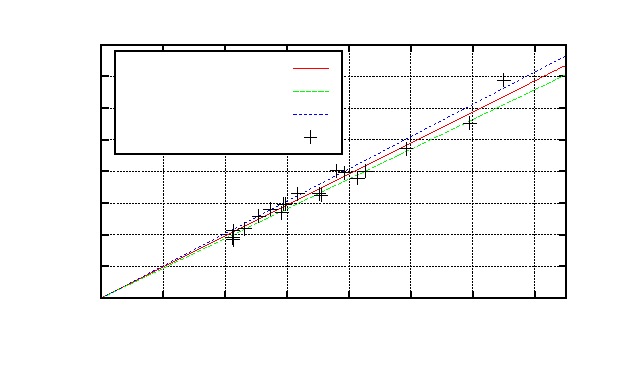
\includegraphics{vattenparabel}}%
    \gplfronttext
  \end{picture}%
\endgroup

\caption{Fokalhöjden över bottnen på en parabel formad av vattenytan i
en roterande skål. Här ges $g$ som lutningen av linjeanpassningen; den
undre och övre linjen svarar mot det minsta respektive största värdet
på $g$ som den uppmätta datan tillåter. Notera också att alla linjer
utgår från origo. }
\label{fig:vattenparabel}
\end{figure}

För att uppskatta felet gör man en huvudanpassnig, men också en övre
och en undre anpassning som sätter en osäkerhetsgräns på lutningen. I
det här fallet ser det som om resultatet från den övre och undre
gränsen blev en osäkerhet på $\Delta{g}=\unit[0,4]{m/s^2}$. Och det
slutgiltiga svaret blir:
\[g=\unit[9,8\pm0,4]{m/s^2}.\]

\paragraph{Anmärkningar}
\begin{enumerate}
\item Även här verkar resultatet stämma, men här är osäkerheten lite
  större än med pendeln. 
\item Glöm inte \textbf{enheter}!
\item Man behöver inte göra livet för krångligt med enheterna. I
  \figref{fig:vattenparabel} är $g$ angiven i enheten $\unit{cm/s^2}$
  för att axlarnas enheter var just $\unit{cm}$ och $\unit{s^2}$. Om
  det sen står att man ska svara i någon annan enhet kan man göra
  enhetsomvandlingen i slutet.
\item Försök göra tabellen så att det blir lätt att se vilka värden
  som ska användas för plottning. I det här fallet mäts $T$ och $h$,
  men ordningen i tabellen är $T$, $(2\omega^2)^{-1}$ och $h$ för att
  det är de två sista som ska användas i plotten. 
\end{enumerate}


\subsection{Diod och serieresistor}
\newcommand{\Vf}{\ensuremath{}V_\text{f}}

En diod är en elektrisk komponent som fungerar som en backventil --
ström kan bara flöda genom den i en riktning. Idealt skulle dioder
kunna betrakts som att ström börjar flyta genom dem så fort spänningen
är positiv. 
Verkliga dioder har dock ett \emph{framspänningsfall} $\Vf$,
vilket betyder att de istället kan approximeras med att strömen börjar
flyta så fort spänningen över dem överstiger $\Vf$.
\begin{quote}
Antag att vi har en svart låda kopplad som i
\figref{fig:LED_schematics}.
Ta reda på resistansen $R$ och framspänningsfallet
$\Vf$, enbart med kännedom om $u$ och $i$.\footnote{Jämför
  detta med finalexperimentet ''LED-karakteristik'' från Wallenbergs
  fysikpris~2015. Mer information om detta finns på 
  \url{https://github.com/andsunds/Fysikpris}, under
  \texttt{Experiment2015/LED/}. } 
\end{quote}

\paragraph{Lösning}
\begin{figure}
\centering
\input{figurer/LED_schematics.pdf_t}
\caption{Kopplingsschema för en diod med en serieresistor. Den
  punktade ramen svarar mot en svart låda.}
\label{fig:LED_schematics}
\end{figure}
Med Kirchhoffs spänningslag fås att (med $u\ge\Vf$)
\begin{equation}
u=\Vf+u_R,
\end{equation}
men Ohms lag säger att $u_R=iR$. Tillsammans ges dessa två uttrycken
ett samband för $i$ som funktion av $u$, $\Vf$ och $R$:
\begin{equation}\label{eq:i}
i=\begin{cases}
0 &, u<\Vf\\
\frac{1}{R}\Big(u-\Vf\Big)&, u\ge\Vf.
\end{cases}
\end{equation}
Alltså ligger $i$ platt $0$ tills $u$ kommer upp till $\Vf$, då börjar den stiga
linjärt med lutning $\nicefrac{1}{R}$. Vi kan alltså finna de
eftersökta storheterna genom att ta reda på linjens lutning och var
den korsar $x$-axeln.

Mäter man ström-spänning-karakteristiken för den svarta lådan får man
ett utseende som i \figref{fig:LED}. Detta ser ut att stämma väl
överens med beskrivningen av \eqref{eq:i}. Notera dock att de
uppmätta mätpunkterna avviker något från linjäranpassningen för de
allra lägsta strömmarna, vlket beror på att den approximationen som
används inte heller är helt korrekt. 

\begin{figure}
\centering
\documentclass[12pt,a4paper]{article}
\pdfoutput=1
%vons grund
\usepackage[utf8]{inputenc}
\usepackage[T1]{fontenc}
\usepackage[swedish]{babel} %OBS! Se till att vi får rätt språk.
\usepackage{amsmath}
\usepackage{lmodern}
\usepackage{units}
\usepackage{icomma}
\usepackage{color}
\usepackage{graphicx}
\usepackage{bbm}
\newcommand{\N}{\ensuremath{\mathbbm{N}}}
\newcommand{\Z}{\ensuremath{\mathbbm{Z}}}
\newcommand{\Q}{\ensuremath{\mathbbm{Q}}}
\newcommand{\R}{\ensuremath{\mathbbm{R}}}
\newcommand{\C}{\ensuremath{\mathbbm{C}}}
\newcommand{\rd}{\ensuremath{\mathrm{d}}}
\newcommand{\id}{\ensuremath{\,\rd}}
\usepackage{hyperref}

%%%%%%%%%%%%%%%%%%%%%%%Egna tillägg%%%%%%%%%%%%%%%%%%%%%%%

%%Partiell derivata
\newcommand{\pd}{\ensuremath{\partial}}
%%Följer ISO-8601 oberoende av språk.
\usepackage{datetime} 
\newdateformat{specialdate}{\THEYEAR-\twodigit{\THEMONTH}-\twodigit{\THEDAY}}
%%Göra grader Celcius
\newcommand{\degC}{\ensuremath{\,^\circ\mathrm{C}}}
%%Figurreferenser
\newcommand{\Figref}{\figurename~\ref} %Stor bokstav i början
\newcommand{\figref}{\MakeLowercase{\figurename}~\ref} 
%%Tabellreferenser
\newcommand{\Tabref}{\tablename~\ref} %Stor bokstav i början
\newcommand{\tabref}{\MakeLowercase{\tablename}~\ref}
%%Ohm enhetskommando
\newcommand{\ohm}{\ifmmode \Omega \else $\Omega$ \fi}
%%Varepsilon är det enda rätta epsilon
\renewcommand{\epsilon}{\varepsilon}


%%%%%%%%%%%%%%%%%%Övriga matnyttiga paket%%%%%%%%%%%%%%%%%

%%För att kunna inkludera andra PDF-dokument
\usepackage{pdfpages}
%%För att kunna ha roterade bilder
\usepackage{rotating}
%%För att inkludera MATLABkod. 
%\usepackage[framed,numbered,autolinebreaks,useliterate]{mcode}
%\usepackage{listings} 
%\lstloadlanguages{matlab} 
%\lstset{language=matlab} 
%\lstset{literate= {å}{{\r{a}}}1 {ä}{{\"a}}1 {ö}{{\"o}}1 {Å}{{\r{A}}}1
%  {Ä}{{\"A}}1 {Ö}{{\"O}}1}%För att få svenska bokstäver från MATLAB.


%%För att själv bestämma marginalerna. 
%\usepackage[
%            top    = 3cm,
%            bottom = 3cm,
%            left   = 3cm, right  = 3cm
%]{geometry}


\usepackage{sectsty}
\sectionfont{\fontsize{13}{0}\selectfont}



\begin{document}
\title{LED-karakteristik}
\author{}
\date{}
\maketitle


% \section*{Bakgrund} 
% Nobelpriset i fysik 2014 gavs till Isamu Akasaki, Hiroshi Amano och
% Shuji Nakamura för deras genombrott med blåa LED:er (Light Emitting
% Diode). Med blåa LED:er blev det plötsligt möjligt att skapa en
% ''vit'' lysdiod. Genom att kombinera röda, gröna och blåa LED:er kan
% man skapa en lysdiod som ser ut att lysa vitt för ögat (jämför en dators
% bildskärm: RGB).

%\section*{Uppgift}
När man ska konstruera en ''vit'' lysdiod kan man ''parallellkoppla''
LED:er av respektive färg. Man måste dock först seriekoppla varje LED
med en resistor innan man kan ''parallellkoppla'' dem, ungefär som i
\figref{svart_låda}.  

\begin{enumerate}
\item Mät upp karakteristiken (ström som funktion av
spänning) för en röd respektive blå LED. Svara med grafer för
respektive LED (kan göras på samma diagram/papper, men du måste
tydligt markera vliken graf som hör till vilken LED).
\item Argumentera utifrån din uppmätta karakteristik vad som skulle
  hända om du försökte parallellkoppla två olika LED:er utan något
  seriemotstånd? 
\end{enumerate}
Till ditt förfogande finns en
''svart låda'' (öppna inte!) med en blå och en röd LED som sticker ut. 
Glöm inte att rita ditt kopplingsschema där även alla mätinstrument
finns med!

\emph{Tips}: En äkta parallellkoppling kännetäcknas av att samma
spänning ligger över båda två av de parallellkopplade komponenterna. 

%föreslå serieresistanser, $R_1$ och $R_2$ enligt
%\figref{parallell},  
%så att en lika stor ström, $i=\unit[5]{mA}$, flyter genom både den
%röda och den blå LED:en om en spänning, $E=\unit[5]{V}$ kopplas in
%i \figref{parallell}. 


% \begin{figure}\centering
% \input{parallell.pdf_t}
% \caption{\label{parallell} En röd och en blå LED ''parallellkopplade''
% med respektive seriemotstånd, $R_1$ och $R_2$ (detta är alltså
% separata komponenter och är inte del av själva LED:erna).}
% \end{figure}



%\newpage
\section*{Materiel}

\begin{itemize}
\item 1 ''Svart låda'' som är kontruerad enligt \figref{svart_låda}.
\item 2 Multimetrar
\item 5 Labbsladdar
\item Milimeterpapper
\end{itemize}


\begin{figure}\centering
\input{svart_lada.pdf_t}
\caption{\label{svart_låda} ''Svart låda''. Du kommer att ha tillgång
  till de två polerna utanför lådan och strömbrytaren för att koppla in den
  blå lysdioden. Du kommer även att kunna se LED:erna för att
  kontrollera ifall de lyser eller inte. }
\end{figure}

\begin{figure}\centering
\centerline{ %centrerar även större bilder
\includegraphics[width=1\textwidth]{../2015/IMG_3590.jpg}
}
%\caption{\label{figuren} Perioden $T$ som funktion av pendellängden.}
\end{figure}

\end{document}





%% På svenska ska citattecknet vara samma i både början och slut.
%% Använd två apostrofer (två enkelfjongar): ''.

%%För att referera till till tidigare fotnot:
%\footnotemark[\value{footnote}]

%% Inkludera PDF-dokument
%\includepdf[pages={1-}]{filnamn.pdf} %Filnamnet får INTE innehålla 'mellanslag'!

%% Figurer inkluderade som pdf-filer
%\begin{figure}\centering
%\centerline{ %centrerar även större bilder
%\includegraphics[width=1\textwidth]{filnamn.pdf}
%}
%\caption{\label{figuren} Perioden $T$ som funktion av pendellängden.}
%\end{figure}

%% Figurer inkluderade med xfigs "Combined PDF/LaTeX"
%\begin{figure}\centering
%\input{filnamn.pdf_t}
%\caption{\label{finafiguren} Perioden $T$ som funktion av
%  pendellängden.}
%\end{figure}


%% Figurer roterade 90 grader
%\begin{sidewaysfigure}\centering
%\centerline{ %centrerar även större bilder
%\includegraphics[width=1\textwidth]{filnamn.pdf}
%}
%\caption{\label{figuren} Perioden $T$ som funktion av pendellängden.}
%\end{sidewaysfigure}

\caption{Ström-spänning-karakteristik för en diod med en serieresistor
som i \figref{fig:LED_schematics}. Linjäranpassningen är gjord efte de
mätpunkter med $u$ från ca 3\,V och uppåt.}
\label{fig:LED}
\end{figure}

Från linjäranpassningen avläses sedan resultaten
\begin{equation*}
\begin{aligned}
\Vf &= \unit[1,8]{V}\\
R &= \unit[1,1]{k\Omega}.
\end{aligned}
\end{equation*}
\paragraph{Anmärkningar} 
\begin{enumerate}
\item Från bygget av uppställnigen vet jag att resistansen skulle vara
  $\unit[1]{k\Omega}$, men toleransen på de resistorerna är 10\,\%. Så
  resistansen verkar stämma.
\item När det gäller att bestämma $\Vf$ är det bättre att använda
  linjäranpassningen hellre än att försöka titta på när man kan börja
  se ström gå. Detta är för att dioden inte riktigt beter sig som i
  modellen precis när den börjar släppa igenom strömmen.
\end{enumerate}


% \subsection{Radioaktivt sönderfall av två silverisotoper}
% Det finns två naturligt förekommande isotoper av silver. Genom att
% bestråla dessa med neutroner kan man skapa två nya, radioaktiva
% isotoper med varsina halveringstider.\footnote{För vidare läsning, se
%   \url{https://github.com/andsunds/Fysikpris} under \texttt{K6}, men
%   du måste själv kompilera \texttt{tex}-filen. (Jag lägger inte upp
%   pdf-filen för att göra trösken att försöka kopiera min rapport något
%   högre.) } 

% \paragraph{Lösning}
% \begin{figure}
% \centering
% % GNUPLOT: LaTeX picture with Postscript
\begingroup
  \makeatletter
  \providecommand\color[2][]{%
    \GenericError{(gnuplot) \space\space\space\@spaces}{%
      Package color not loaded in conjunction with
      terminal option `colourtext'%
    }{See the gnuplot documentation for explanation.%
    }{Either use 'blacktext' in gnuplot or load the package
      color.sty in LaTeX.}%
    \renewcommand\color[2][]{}%
  }%
  \providecommand\includegraphics[2][]{%
    \GenericError{(gnuplot) \space\space\space\@spaces}{%
      Package graphicx or graphics not loaded%
    }{See the gnuplot documentation for explanation.%
    }{The gnuplot epslatex terminal needs graphicx.sty or graphics.sty.}%
    \renewcommand\includegraphics[2][]{}%
  }%
  \providecommand\rotatebox[2]{#2}%
  \@ifundefined{ifGPcolor}{%
    \newif\ifGPcolor
    \GPcolortrue
  }{}%
  \@ifundefined{ifGPblacktext}{%
    \newif\ifGPblacktext
    \GPblacktexttrue
  }{}%
  % define a \g@addto@macro without @ in the name:
  \let\gplgaddtomacro\g@addto@macro
  % define empty templates for all commands taking text:
  \gdef\gplbacktext{}%
  \gdef\gplfronttext{}%
  \makeatother
  \ifGPblacktext
    % no textcolor at all
    \def\colorrgb#1{}%
    \def\colorgray#1{}%
  \else
    % gray or color?
    \ifGPcolor
      \def\colorrgb#1{\color[rgb]{#1}}%
      \def\colorgray#1{\color[gray]{#1}}%
      \expandafter\def\csname LTw\endcsname{\color{white}}%
      \expandafter\def\csname LTb\endcsname{\color{black}}%
      \expandafter\def\csname LTa\endcsname{\color{black}}%
      \expandafter\def\csname LT0\endcsname{\color[rgb]{1,0,0}}%
      \expandafter\def\csname LT1\endcsname{\color[rgb]{0,1,0}}%
      \expandafter\def\csname LT2\endcsname{\color[rgb]{0,0,1}}%
      \expandafter\def\csname LT3\endcsname{\color[rgb]{1,0,1}}%
      \expandafter\def\csname LT4\endcsname{\color[rgb]{0,1,1}}%
      \expandafter\def\csname LT5\endcsname{\color[rgb]{1,1,0}}%
      \expandafter\def\csname LT6\endcsname{\color[rgb]{0,0,0}}%
      \expandafter\def\csname LT7\endcsname{\color[rgb]{1,0.3,0}}%
      \expandafter\def\csname LT8\endcsname{\color[rgb]{0.5,0.5,0.5}}%
    \else
      % gray
      \def\colorrgb#1{\color{black}}%
      \def\colorgray#1{\color[gray]{#1}}%
      \expandafter\def\csname LTw\endcsname{\color{white}}%
      \expandafter\def\csname LTb\endcsname{\color{black}}%
      \expandafter\def\csname LTa\endcsname{\color{black}}%
      \expandafter\def\csname LT0\endcsname{\color{black}}%
      \expandafter\def\csname LT1\endcsname{\color{black}}%
      \expandafter\def\csname LT2\endcsname{\color{black}}%
      \expandafter\def\csname LT3\endcsname{\color{black}}%
      \expandafter\def\csname LT4\endcsname{\color{black}}%
      \expandafter\def\csname LT5\endcsname{\color{black}}%
      \expandafter\def\csname LT6\endcsname{\color{black}}%
      \expandafter\def\csname LT7\endcsname{\color{black}}%
      \expandafter\def\csname LT8\endcsname{\color{black}}%
    \fi
  \fi
  \setlength{\unitlength}{0.0500bp}%
  \begin{picture}(6802.00,3968.00)%
    \gplgaddtomacro\gplbacktext{%
      \csname LTb\endcsname%
      \put(814,1326){\makebox(0,0)[r]{\strut{}$10^{2}$}}%
      \csname LTb\endcsname%
      \put(814,2514){\makebox(0,0)[r]{\strut{}$10^{3}$}}%
      \csname LTb\endcsname%
      \put(814,3703){\makebox(0,0)[r]{\strut{}$10^{4}$}}%
      \csname LTb\endcsname%
      \put(946,484){\makebox(0,0){\strut{} 0}}%
      \csname LTb\endcsname%
      \put(1674,484){\makebox(0,0){\strut{} 2}}%
      \csname LTb\endcsname%
      \put(2402,484){\makebox(0,0){\strut{} 4}}%
      \csname LTb\endcsname%
      \put(3130,484){\makebox(0,0){\strut{} 6}}%
      \csname LTb\endcsname%
      \put(3857,484){\makebox(0,0){\strut{} 8}}%
      \csname LTb\endcsname%
      \put(4585,484){\makebox(0,0){\strut{} 10}}%
      \csname LTb\endcsname%
      \put(5313,484){\makebox(0,0){\strut{} 12}}%
      \csname LTb\endcsname%
      \put(6041,484){\makebox(0,0){\strut{} 14}}%
      \put(176,2203){\rotatebox{-270}{\makebox(0,0){\strut{}$A$ /[sönderfall/min]}}}%
      \put(3675,154){\makebox(0,0){\strut{}$t$ /[min.]}}%
    }%
    \gplgaddtomacro\gplfronttext{%
      \csname LTb\endcsname%
      \put(5682,3486){\makebox(0,0)[r]{\strut{}Uppmätt data}}%
      \csname LTb\endcsname%
      \put(5682,3266){\makebox(0,0)[r]{\strut{}Anpassing $^{108}$Ag}}%
      \csname LTb\endcsname%
      \put(5682,3046){\makebox(0,0)[r]{\strut{}Korrigerad data}}%
      \csname LTb\endcsname%
      \put(5682,2826){\makebox(0,0)[r]{\strut{}Anpassning $^{110}$Ag}}%
      \csname LTb\endcsname%
      \put(5682,2606){\makebox(0,0)[r]{\strut{}Anpassing tillsammans}}%
    }%
    \gplbacktext
    \put(0,0){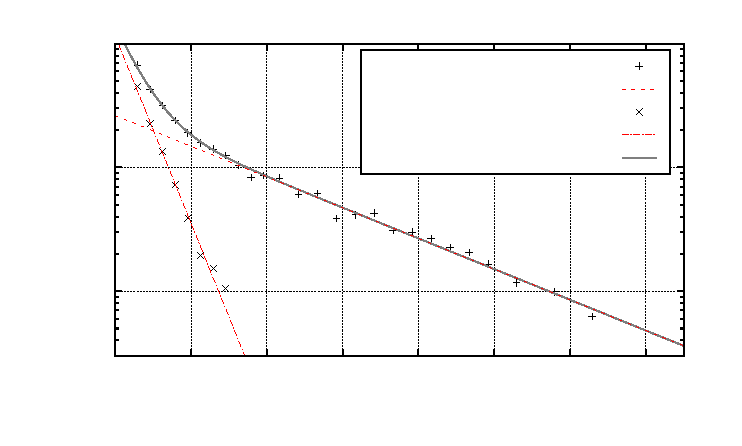
\includegraphics{silverisotoper}}%
    \gplfronttext
  \end{picture}%
\endgroup

% \caption{}
% \label{fig:silverisotoper}
% \end{figure}

\newpage
\section{Sammanfattning}
Det finns många saker att tänka på när man ska göra
experiment. Felanalys är en av dem, men i grund och botten är det inte
mer än två eller tre formler att kunna. 
\\[16pt]
Den första formeln är den för standardfelet i medelvärdet
\[
\Delta{x} = \frac{s}{\sqrt{N}} 
= \frac{1}{\sqrt{N}}\sqrt{\frac{1}{N-1}\sum_{i=1}^N (x_i-\bar{x})^2}.
\]
Den ska användas för att beräkna osäkerheten i ett medelvärde
($\bar{x}$) av upprepade mätningar ($x_i$) av någon storhet. Det finns
även inbyggt i många lite mer avancerade miniränkare att automatiskt
räkna ut $s$ från en serie inmatade värden. Kom bara ihåg att dela med
$\sqrt{N}$. 
\\[16pt]
Sen är det formeln för hur man propagerar fel från uppmätta variabler
genom ett samband. Osäkerheten i den uträknade parametern blir då
\[
\Delta{G} \approx \sqrt{
\left(\pdv{G}{x}\Delta{x}\right)^2
+\left(\pdv{G}{y}\Delta{y}\right)^2
+\left(\pdv{G}{z}\Delta{z}\right)^2
}.
\]
Den här formeln ska användas om man har något godtyckligt samband
mellan de uppmätta storheterna ($x$, $y$ och $z$) och slutparametern
som söks ($G$). Om det däremot rör sig om ett potenssamband kan man
använda den lite enklare formeln:
\[
\frac{\Delta{G}}{\bar{G}} \approx \sqrt{
\left(\alpha\,\frac{\Delta{x}}{\bar{x}}\right)^2
+\left(\beta\,\frac{\Delta{y}}{\bar{y}}\right)^2
+\left(\gamma\,\frac{\Delta{z}}{\bar{z}}\right)^2
},
\]
där $\alpha$, $\beta$ och $\gamma$ är exponenterna på $x$, $y$
respektive $z$.
\\[16pt]
Det sista man ska ta med sig härifrån är att om man tar upp en
mätserie är det bra om man kan försöka plotta upp sin mätdata på ett
sätt så att man får linjära samband. De är oftast enkare att hantera. 




%\newpage
%\bibliographystyle{ieeetr}
%\bibliography{referenser}%kräver en fil som heter 'referenser.bib'          
\clearpage
\appendix

% \section{Hur man använder miniräknaren för statistik}
% \label{sec:calculator}
% Det här en kort guide i hur man kan använda sin
% IPhO-miniräknare\footnotemark{}

% \footnotetext{Jag har tillgång till mina två olika IPhO-miniräknare:
%   \texttt{Casio~fx-82MS} och \texttt{HP~10s+}. Guiden gäller för dessa
% ock liknande modeller (tyvärr har \texttt{TI-30~ECO~RS} ett lite
% annorlunda gränssnitt).}



\section{Taylorutvecklingar}\label{sec:Taylor}
\begin{figure}
\centering
% GNUPLOT: LaTeX picture with Postscript
\begingroup
  \makeatletter
  \providecommand\color[2][]{%
    \GenericError{(gnuplot) \space\space\space\@spaces}{%
      Package color not loaded in conjunction with
      terminal option `colourtext'%
    }{See the gnuplot documentation for explanation.%
    }{Either use 'blacktext' in gnuplot or load the package
      color.sty in LaTeX.}%
    \renewcommand\color[2][]{}%
  }%
  \providecommand\includegraphics[2][]{%
    \GenericError{(gnuplot) \space\space\space\@spaces}{%
      Package graphicx or graphics not loaded%
    }{See the gnuplot documentation for explanation.%
    }{The gnuplot epslatex terminal needs graphicx.sty or graphics.sty.}%
    \renewcommand\includegraphics[2][]{}%
  }%
  \providecommand\rotatebox[2]{#2}%
  \@ifundefined{ifGPcolor}{%
    \newif\ifGPcolor
    \GPcolortrue
  }{}%
  \@ifundefined{ifGPblacktext}{%
    \newif\ifGPblacktext
    \GPblacktexttrue
  }{}%
  % define a \g@addto@macro without @ in the name:
  \let\gplgaddtomacro\g@addto@macro
  % define empty templates for all commands taking text:
  \gdef\gplbacktext{}%
  \gdef\gplfronttext{}%
  \makeatother
  \ifGPblacktext
    % no textcolor at all
    \def\colorrgb#1{}%
    \def\colorgray#1{}%
  \else
    % gray or color?
    \ifGPcolor
      \def\colorrgb#1{\color[rgb]{#1}}%
      \def\colorgray#1{\color[gray]{#1}}%
      \expandafter\def\csname LTw\endcsname{\color{white}}%
      \expandafter\def\csname LTb\endcsname{\color{black}}%
      \expandafter\def\csname LTa\endcsname{\color{black}}%
      \expandafter\def\csname LT0\endcsname{\color[rgb]{1,0,0}}%
      \expandafter\def\csname LT1\endcsname{\color[rgb]{0,1,0}}%
      \expandafter\def\csname LT2\endcsname{\color[rgb]{0,0,1}}%
      \expandafter\def\csname LT3\endcsname{\color[rgb]{1,0,1}}%
      \expandafter\def\csname LT4\endcsname{\color[rgb]{0,1,1}}%
      \expandafter\def\csname LT5\endcsname{\color[rgb]{1,1,0}}%
      \expandafter\def\csname LT6\endcsname{\color[rgb]{0,0,0}}%
      \expandafter\def\csname LT7\endcsname{\color[rgb]{1,0.3,0}}%
      \expandafter\def\csname LT8\endcsname{\color[rgb]{0.5,0.5,0.5}}%
    \else
      % gray
      \def\colorrgb#1{\color{black}}%
      \def\colorgray#1{\color[gray]{#1}}%
      \expandafter\def\csname LTw\endcsname{\color{white}}%
      \expandafter\def\csname LTb\endcsname{\color{black}}%
      \expandafter\def\csname LTa\endcsname{\color{black}}%
      \expandafter\def\csname LT0\endcsname{\color{black}}%
      \expandafter\def\csname LT1\endcsname{\color{black}}%
      \expandafter\def\csname LT2\endcsname{\color{black}}%
      \expandafter\def\csname LT3\endcsname{\color{black}}%
      \expandafter\def\csname LT4\endcsname{\color{black}}%
      \expandafter\def\csname LT5\endcsname{\color{black}}%
      \expandafter\def\csname LT6\endcsname{\color{black}}%
      \expandafter\def\csname LT7\endcsname{\color{black}}%
      \expandafter\def\csname LT8\endcsname{\color{black}}%
    \fi
  \fi
  \setlength{\unitlength}{0.0500bp}%
  \begin{picture}(6802.00,3968.00)%
    \gplgaddtomacro\gplbacktext{%
      \csname LTb\endcsname%
      \put(462,704){\makebox(0,0)[r]{\strut{}-2}}%
      \csname LTb\endcsname%
      \put(462,1316){\makebox(0,0)[r]{\strut{}-1}}%
      \csname LTb\endcsname%
      \put(462,1929){\makebox(0,0)[r]{\strut{} 0}}%
      \csname LTb\endcsname%
      \put(462,2541){\makebox(0,0)[r]{\strut{} 1}}%
      \csname LTb\endcsname%
      \put(462,3153){\makebox(0,0)[r]{\strut{} 2}}%
      \csname LTb\endcsname%
      \put(594,484){\makebox(0,0){\strut{}-4}}%
      \csname LTb\endcsname%
      \put(1320,484){\makebox(0,0){\strut{}-3}}%
      \csname LTb\endcsname%
      \put(2047,484){\makebox(0,0){\strut{}-2}}%
      \csname LTb\endcsname%
      \put(2773,484){\makebox(0,0){\strut{}-1}}%
      \csname LTb\endcsname%
      \put(3500,484){\makebox(0,0){\strut{} 0}}%
      \csname LTb\endcsname%
      \put(4226,484){\makebox(0,0){\strut{} 1}}%
      \csname LTb\endcsname%
      \put(4952,484){\makebox(0,0){\strut{} 2}}%
      \csname LTb\endcsname%
      \put(5679,484){\makebox(0,0){\strut{} 3}}%
      \csname LTb\endcsname%
      \put(6405,484){\makebox(0,0){\strut{} 4}}%
      \put(3499,154){\makebox(0,0){\strut{}\Large$x$}}%
    }%
    \gplgaddtomacro\gplfronttext{%
      \csname LTb\endcsname%
      \put(2908,3740){\makebox(0,0)[r]{\strut{}$\sin(x)$}}%
      \csname LTb\endcsname%
      \put(2908,3520){\makebox(0,0)[r]{\strut{}$x$}}%
      \csname LTb\endcsname%
      \put(5083,3740){\makebox(0,0)[r]{\strut{}$x - \nicefrac{x^3}{6}$}}%
      \csname LTb\endcsname%
      \put(5083,3520){\makebox(0,0)[r]{\strut{}$x - \nicefrac{x^3}{6} + \nicefrac{x^5}{120}$}}%
    }%
    \gplbacktext
    \put(0,0){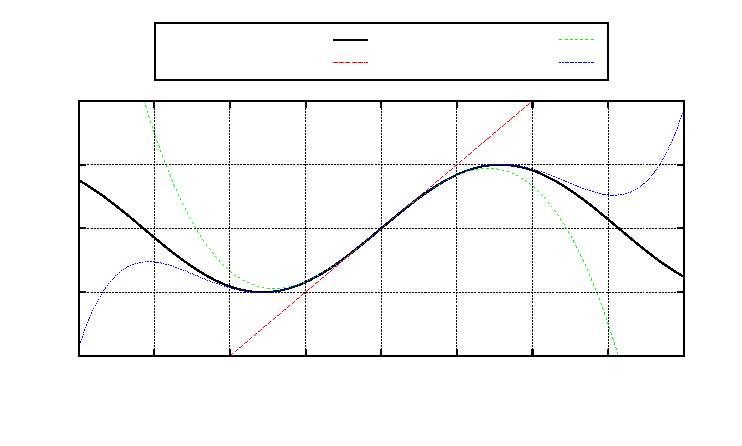
\includegraphics{taylor_sin}}%
    \gplfronttext
  \end{picture}%
\endgroup

\caption{}
\label{fig:taylor_sin}
\end{figure}

Ibland är det svårt att hantera exakta uttryck, antingen för att de är
jobbiga att beräkna numeriskt eller att de lätt blir vädigt svåra att
hantera matematiskt. Därför är det nyttigt att kunna approximera. En
av de vanligaste approximationerna som används i fysiken är
Taylorutvecklingar\footnotemark{}. De används för att approximera
funktioner med polynom av olika hög grad, Taylorpolynomen. Till
exempel visar \figref{fig:taylor_sin} de tre första (unika)
Taylorpolynomen för $\sin(x)$ kring $x=0$.
\footnotetext{Mer eller mindre all fysik bygger på en Taylorutveckling
någonstans. Ett extremfal är Newtonsk mekanik som egentligen bara är en
första ordningens Taylorutveckling av Einsteins relativitetsteori. }

Har man en funktion $f$ (som är tillräckligt många gånger deriverbar)
kan man uttrycka den $n$:te ordningens Taylorpolynom, $p_n$, kring punkten
$a$ som:
\begin{equation}
\begin{aligned}
p_n(x) =& f(a) + f'(a)\,(x-a) + \frac{1}{2} f''(a)\,(x-a)^2 
 + \frac{1}{6} f^{(3)}(a)(x-a)^3 + \ldots\\
 & \ldots + \frac{1}{n!}f^{(n)}(a)\,(x-a)^n\\
=& \sum_{i=0}^{n} \frac{f^{(i)}(x-a)^i}{i!}.
\end{aligned}
\end{equation}
Ju fler termer som tas med destu bättre blir approximationen, men
destu snårigare blir också uttrycket. 
Oftas nöjer man sig dock med första ordningens
Taylorutveckling/Taylorpolynom, vilket är samma som att
linjärapproximera funktionen med dess tangent:
\begin{equation}
p_1(x) = f(a) + f'(a)\,(x-a).
\end{equation}

En trevlig sak med att göra en linjärapproximation är att uttrycket
$\nicefrac{\Delta{p_1}}{\Delta{x}}$ blir samma som derivatan
$f'(a)$. Med andra ord så är 
\begin{equation}
f'(a)\,\Delta{x} = \Delta{p_1} \approx \Delta{f}.
\end{equation}
Detta kan användas för att uppskatta osäkerheten i ett beräknat uttryck,
$f$, givet osäkerheten i inparametern, $x$.

\end{document}

